% A simple template for Beamer presentations in LaTeX
% 
% To produce pdf run:
%   $ pdflatex beamer.tex 

\documentclass{beamer}
%\usetheme{Singapore}
\usetheme{Boadilla}

% Bibliography
%\usepackage{cite}
\usepackage{biblatex}

\hypersetup{colorlinks=true}

% Show table of contents between sections
\AtBeginSection[]
{
  \begin{frame}
    \frametitle{Table of Contents}
    \tableofcontents[currentsection]
  \end{frame}
}

% Graphics examples
%\centerline{\includegraphics[height=2.5in]{figs/normal.pdf}}
%\includegraphics[width=4in]{figs/makefile.png}

%%%%%%%%%%%%%%%%%%%%%%%%%%%%%%%%%%%%%%%%%%%%%%%%%%%%%%%%%%%%

\begin{document}

\title{Parallel Computing Through Code Analysis}
\date{\today}
\date{10 May 2017}
\author{Clark Fitzgerald}
\institute{UC Davis}
\titlegraphic{\includegraphics[height=.5\textheight]{../workflow.pdf}}

\frame{\titlepage}

%\begin{frame}
%    \frametitle{Outline}
%    \tableofcontents
%\end{frame}

%%%%%%%%%%%%%%%%%%%%%%%%%%%%%%%%%%%%%%%%%%%%%%%%%%%%%%%%%%%%
\section{Introduction}
%%%%%%%%%%%%%%%%%%%%%%%%%%%%%%%%%%%%%%%%%%%%%%%%%%%%%%%%%%%%
\begin{frame}

\frametitle{Modern platforms provide incredible computing power.}

% I'm showing Hadoop, but it could be any cluster.

\begin{figure}
            %\hfill
            
\includegraphics[width=1.3in]{macbook.jpg}
            %\hfill
            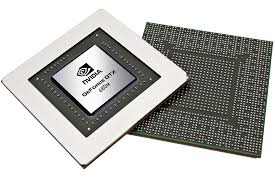
\includegraphics[width=1.3in]{gpu.jpg}
            %\hfill
\end{figure}
\begin{figure}
            %\hfill
            
\includegraphics[width=1.3in]{spark.png}
            %\hfill
            
\includegraphics[width=1.3in]{aws.png}
            %\hfill
\end{figure}

\pause 

But they require expertise.

\end{frame}
%%%%%%%%%%%%%%%%%%%%%%%%%%%%%%%%%%%%%%%%%%%%%%%%%%%%%%%%%%%%
\begin{frame}

    \frametitle{The broader goal is for users to write higher level code
    that also performs better.}

    \begin{itemize}
        \item Parallel programming is a means to this end
        \item Compilation is another way
    \end{itemize}

\end{frame}
%%%%%%%%%%%%%%%%%%%%%%%%%%%%%%%%%%%%%%%%%%%%%%%%%%%%%%%%%%%%
\begin{frame}

    % TODO: better title
    \frametitle{We take a holistic approach to the computation.}

\centerline{\includegraphics[width=.8\textwidth]{../workflow.pdf}}

%In contrast, compilation can only examine the code.

\end{frame}
%%%%%%%%%%%%%%%%%%%%%%%%%%%%%%%%%%%%%%%%%%%%%%%%%%%%%%%%%%%%
\begin{frame}

    \frametitle{The R language offers several benefits.}

\centerline{
\includegraphics[height=1in]{Rlogo.png}}

    \begin{itemize}
        \item Functional languages simplify parallel computing
        \item R is widely used for statistics and data analysis
        \item R supports metaprogramming aka ``programming on the
            language''
    \end{itemize}

\end{frame}
%%%%%%%%%%%%%%%%%%%%%%%%%%%%%%%%%%%%%%%%%%%%%%%%%%%%%%%%%%%%
\section{Motivating Example}
%%%%%%%%%%%%%%%%%%%%%%%%%%%%%%%%%%%%%%%%%%%%%%%%%%%%%%%%%%%%
\begin{frame}

    \frametitle{The purpose of this example is to motivate the proposed
    research.}

    \begin{itemize}
        \item Working with Professor Michael Zhang from Civil Engineering
        \item Illustrates complexity when computing with larger data sets
    \end{itemize}

\end{frame}
%%%%%%%%%%%%%%%%%%%%%%%%%%%%%%%%%%%%%%%%%%%%%%%%%%%%%%%%%%%%
\begin{frame}

    \frametitle{Loop detectors count vehicle flow, measuring velocity and
    density (time sensor is activated).}

\centerline{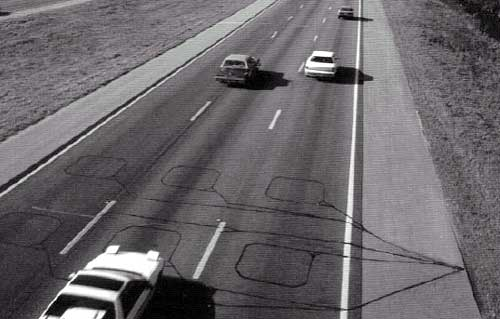
\includegraphics[height=2.5in]{loop_detector.jpg}}

\end{frame}
%%%%%%%%%%%%%%%%%%%%%%%%%%%%%%%%%%%%%%%%%%%%%%%%%%%%%%%%%%%%
\begin{frame}

\frametitle{Caltrans Performance Measurement System (PeMS) records loop
    detector
data for the whole state.}

    \begin{itemize}
        \item Each sensor measures 3 quantities
        \item Data point every 30 seconds
        \item $43,680$ sensors in California
        \item $\implies$  377 million data points per day
    \end{itemize}

\end{frame}
%%%%%%%%%%%%%%%%%%%%%%%%%%%%%%%%%%%%%%%%%%%%%%%%%%%%%%%%%%%%
\begin{frame}

    \frametitle{The \emph{fundamental diagram} in traffic engineering shows
        the relationship between flow and density.}

    \centerline{\includegraphics[height=2.5in]{../../analysis/pems/occ_flow_with_sample.pdf}}

\end{frame}
%%%%%%%%%%%%%%%%%%%%%%%%%%%%%%%%%%%%%%%%%%%%%%%%%%%%%%%%%%%%
\begin{frame}

    \frametitle{Each station has a fundamental diagram, which can be fit in
    parallel.}

\centerline{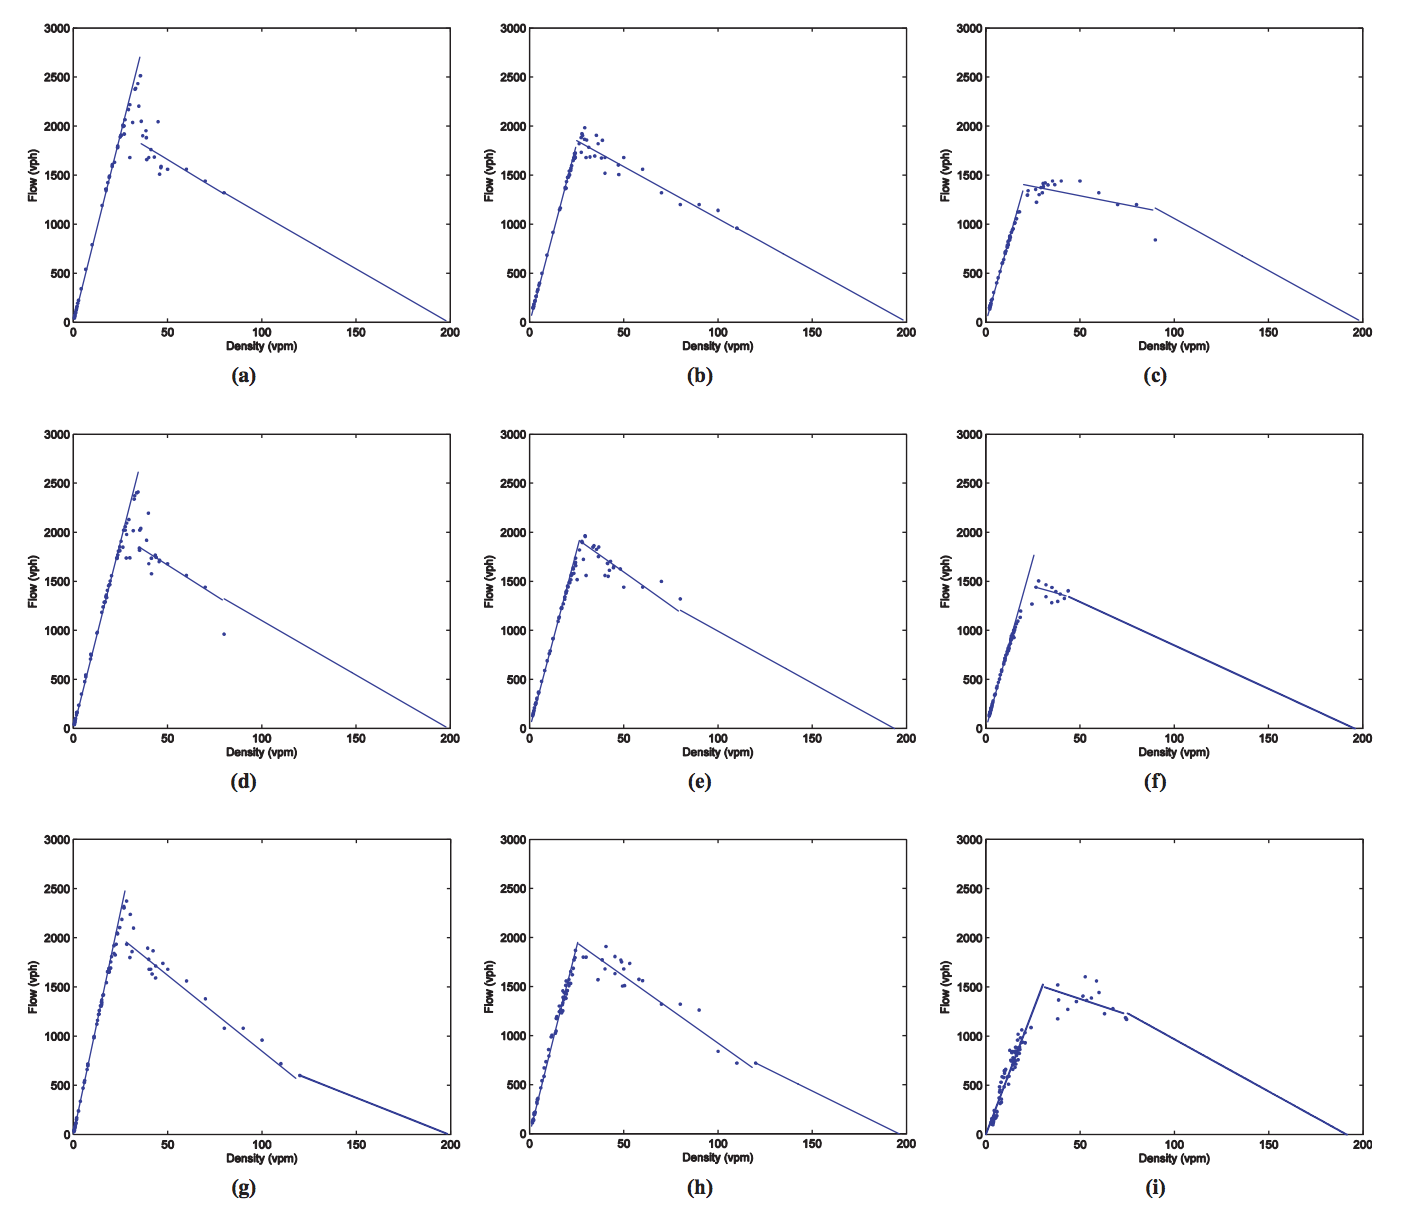
\includegraphics[height=2.5in]{many_fundamental_diagram.png}}

Source: Li, Zhang 2011

\end{frame}
%%%%%%%%%%%%%%%%%%%%%%%%%%%%%%%%%%%%%%%%%%%%%%%%%%%%%%%%%%%%
\begin{frame}

    \frametitle{Using more data allows new types of analyses.}

    % Policy is especially interesting, because that can potentially be changed
    % Recommending state wide policy, then why not look at data for the
    % whole state?

    \begin{itemize}
        \item Effect of policy such as speed limits and carpool lanes
        \item Impact of road features such as on/off ramps
        \item Effect of weather
        \item Clustering detectors
    \end{itemize}

\end{frame}
%%%%%%%%%%%%%%%%%%%%%%%%%%%%%%%%%%%%%%%%%%%%%%%%%%%%%%%%%%%%
\begin{frame}[fragile]

    \frametitle{R expresses statistical computation well.}

% This is a good reason to stay with R

    \centerline{\includegraphics[height=1in]{../../analysis/pems/occ_flow_with_sample.pdf}}

\begin{verbatim}
by(data=single_day, INDICES = station, FUN = my_rlm)
\end{verbatim}

    \begin{itemize}
        \item For a single day with 377 million observations this can be
            done on a single machine.
        \item A sensible way to run this in parallel is to \texttt{fork()}
            the process after reading in the data.
        \item So you write a bunch of code to do that :)
    \end{itemize}

\end{frame}
%%%%%%%%%%%%%%%%%%%%%%%%%%%%%%%%%%%%%%%%%%%%%%%%%%%%%%%%%%%%
\begin{frame}[fragile]

    \frametitle{Small changes can totally change the
    computation.}

% The following code is for illustrative purposes only, it doesn't run

    If we compute on one year then this will exceed memory.

\begin{verbatim}
by(data=one_year, INDICES = station, FUN = my_rlm)
\end{verbatim}

\pause 

    A different model, such as least squares, may be able to process the
    data as a stream.

\begin{verbatim}
by(data=one_year, INDICES = station, FUN = my_lm)
\end{verbatim}

\end{frame}
%%%%%%%%%%%%%%%%%%%%%%%%%%%%%%%%%%%%%%%%%%%%%%%%%%%%%%%%%%%%
\begin{frame}[fragile]

    \frametitle{Access to the underlying database may allow us to run code directly inside the
    database.}

\begin{verbatim}
SELECT station, my_rlm(...) FROM data GROUP BY station
\end{verbatim}


%\end{frame}
%%%%%%%%%%%%%%%%%%%%%%%%%%%%%%%%%%%%%%%%%%%%%%%%%%%%%%%%%%%%%
%\begin{frame}
%
%    \frametitle{Lets scale up the computations with parallel programming}
%
%    \begin{itemize}
%        \item Several parallel strategies exist to improve performance
%        \item Which is best depends on the platform and data
%        \item Each one requires deeper knowledge of that particular technology
%        \item Therefore techniques to programmatically identify and use the parallel
%  patterns implicit in code would be valuable
%    \end{itemize}

\end{frame}
%%%%%%%%%%%%%%%%%%%%%%%%%%%%%%%%%%%%%%%%%%%%%%%%%%%%%%%%%%%%
\section{Parallel Concepts}
%%%%%%%%%%%%%%%%%%%%%%%%%%%%%%%%%%%%%%%%%%%%%%%%%%%%%%%%%%%%
\begin{frame}[fragile]

\frametitle{This simple example shows how to write parallel code in R.}

% This creates an intermediate vector of length n.
% Fails when n approaches limits of memory.

Consider computing the mean,

\begin{equation}
    \bar{x} = \frac{1}{n} \sum_{i = 1}^n x_i
\label{eq:mean}
\end{equation}

where the $x_i$'s are i.i.d. $\sim t(d)$. 
    
In R this code is written:

\begin{verbatim}
xbar = mean(rt(n, d))
\end{verbatim}

\end{frame}
%%%%%%%%%%%%%%%%%%%%%%%%%%%%%%%%%%%%%%%%%%%%%%%%%%%%%%%%%%%%
\begin{frame}

    \frametitle{We can express the mean as a weighted mean.}

Suppose $n = n_j p$, where $n_j$ is the chunk size and $p$ is the number of
chunks.

\begin{equation}
    \bar{x} = \frac{1}{n} \sum_{j = 1}^p \sum_{i = 1}^{n_j} x_{ij}
    = \frac{1}{p} \sum_{j = 1}^p \frac{1}{n_j} \sum_{i = 1}^{n_j} x_{ij}
    = \frac{1}{p} \sum_{j = 1}^p \bar{x}_{\cdot j}
\label{eq:mean_partial}
\end{equation}

\end{frame}
%%%%%%%%%%%%%%%%%%%%%%%%%%%%%%%%%%%%%%%%%%%%%%%%%%%%%%%%%%%%
\begin{frame}[fragile]

    \frametitle{The weighted mean can be directly translated into R code.}

\begin{verbatim}

partial_means = replicate(p, mean(rt(n_j, d)))
xbar = mean(partial_means)

\end{verbatim}

\pause 

    \begin{itemize}
        \item While not parallel, this effectively removes the memory limits.
        \item How to choose the $n_j$ and $p$?
    \end{itemize}

\end{frame}
%%%%%%%%%%%%%%%%%%%%%%%%%%%%%%%%%%%%%%%%%%%%%%%%%%%%%%%%%%%%
\begin{frame}

    \frametitle{The same computation can be evaluated on many workers
    simultaneously.}

\centerline{\includegraphics[height=3in]{../snow.pdf}}

\end{frame}
%%%%%%%%%%%%%%%%%%%%%%%%%%%%%%%%%%%%%%%%%%%%%%%%%%%%%%%%%%%%
\begin{frame}[fragile]

    \frametitle{Here is one way to parallelize this code.}

\begin{verbatim}
library(parallel)
p = floor(detectCores(logical = FALSE) / 2)
n_j = n / p
cluster = makeCluster(p)
clusterExport(cluster, c("n_j", "p"))
partial_means = unlist(
    clusterEvalQ(cluster, mean(rt(n_j, p))))
xbar = mean(partial_means)
\end{verbatim}

\end{frame}
%%%%%%%%%%%%%%%%%%%%%%%%%%%%%%%%%%%%%%%%%%%%%%%%%%%%%%%%%%%%
\begin{frame}[fragile]

    \frametitle{We're considering a system that transforms expressions.}

    Input:

\begin{verbatim}
xbar = mean(rt(n, d))
\end{verbatim}

    Output (omitting boilerplate):

\begin{verbatim}
p = floor(detectCores(logical = FALSE) / 2)
partial_means = clusterEvalQ(cluster, mean(rt(n_j, p)))
xbar = mean(partial_means)
\end{verbatim}

\end{frame}
%%%%%%%%%%%%%%%%%%%%%%%%%%%%%%%%%%%%%%%%%%%%%%%%%%%%%%%%%%%%
\begin{frame}[fragile]

    \frametitle{This can be difficult because R is implemented in C.}

\begin{verbatim}
> rt
function (n, df, ncp)
{
    if (missing(ncp))
        .Call(C_rt, n, df)
    else ...
\end{verbatim}

\pause

    Options:

    \begin{itemize}
        \item Start from \texttt{replicate(p, mean(rnorm(n\_j)))}
        \item Allow users to indicate how \texttt{rt} is vectorized
        \item Analyze the preprocessed C code
        \item Rewrite the C code in R, then analyze the R code
    \end{itemize}

\end{frame}
%%%%%%%%%%%%%%%%%%%%%%%%%%%%%%%%%%%%%%%%%%%%%%%%%%%%%%%%%%%%
\section{Code Analysis}
%%%%%%%%%%%%%%%%%%%%%%%%%%%%%%%%%%%%%%%%%%%%%%%%%%%%%%%%%%%%
\begin{frame}

    \frametitle{\{Code, Data, Platform\} together determine the execution
    strategy.}

\begin{figure}
            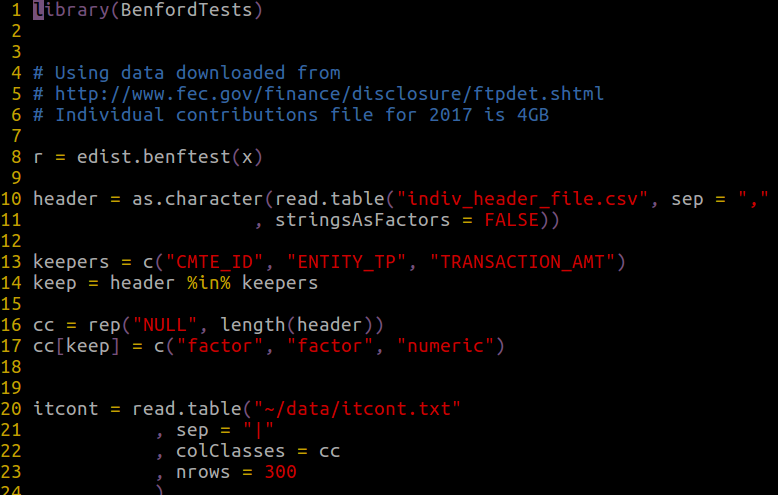
\includegraphics[width=1.4in]{code_screen.png}
            \hfill
            
\includegraphics[width=1in]{database.png}
            \hfill
            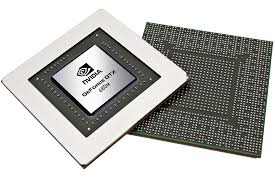
\includegraphics[width=1.4in]{gpu.jpg}
\end{figure}

%    \begin{itemize}
%    \item \textbf{Code} script to be executed
%    \item \textbf{Data} in-memory, files, database, etc
%    \item \textbf{Platform} 4 core laptop, server with GPU, Spark cluster,
%        etc
%    \end{itemize}

\end{frame}
%%%%%%%%%%%%%%%%%%%%%%%%%%%%%%%%%%%%%%%%%%%%%%%%%%%%%%%%%%%%
\begin{frame}[fragile]

    \frametitle{CodeDepends is a tool for analyzing code as a data
    structure.}

    Consider the following script:

\begin{verbatim}
params = read.csv('params.csv')
data = read.csv('data.csv')
sim = simulate(params, 1000000)
joined = merge(data, sim)
\end{verbatim}

\end{frame}
%%%%%%%%%%%%%%%%%%%%%%%%%%%%%%%%%%%%%%%%%%%%%%%%%%%%%%%%%%%%
\begin{frame}

    \frametitle{The expression graph represents the dependencies between
    expressions.}

    \centerline{\includegraphics[height=2.5in]{../codegraph.pdf}}

\end{frame}
%%%%%%%%%%%%%%%%%%%%%%%%%%%%%%%%%%%%%%%%%%%%%%%%%%%%%%%%%%%%
\begin{frame}


\frametitle{Is it worth it to go parallel?}

    \centerline{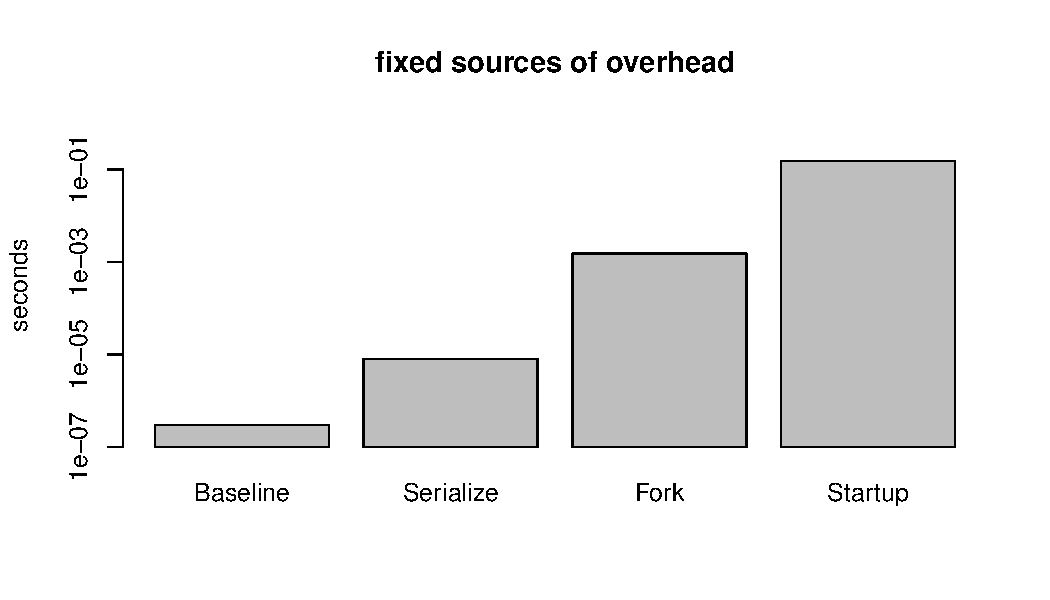
\includegraphics[height=2.5in]{../compute_times/overhead}}

% This has to be answered for every piece of code, every time

% If there wasn't any overhead, we would use it all the time for
% everything.

% If you start up a process, you want to keep it around

\end{frame}
%%%%%%%%%%%%%%%%%%%%%%%%%%%%%%%%%%%%%%%%%%%%%%%%%%%%%%%%%%%%
\begin{frame}

\frametitle{Given an existing SNOW cluster with 2 workers we see benefits
    from parallelization when $n > 4000$.}

\centerline{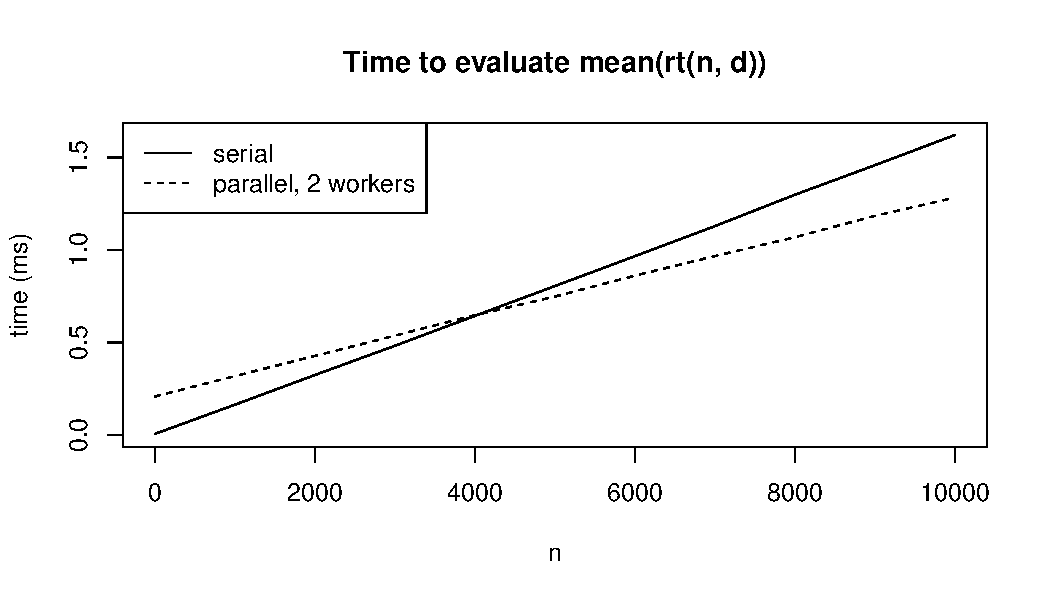
\includegraphics[height=2.5in]{../compute_times/ser_vs_par.pdf}}

Timings on a 3.4 GHz Intel i3 CPU

\end{frame}
%%%%%%%%%%%%%%%%%%%%%%%%%%%%%%%%%%%%%%%%%%%%%%%%%%%%%%%%%%%%
\begin{frame}

    \frametitle{Factors to consider}

\textbf{Parameters}
\begin{itemize}
    \item number of processor cores to use
    \item size of each chunk
    \item which functions to combine in one processing step
\end{itemize}

\textbf{Constraints}
\begin{itemize}
    \item number of cores available
    \item network bandwidth
    \item disk IO speed
    \item available memory
\end{itemize}

%\end{frame}
%%%%%%%%%%%%%%%%%%%%%%%%%%%%%%%%%%%%%%%%%%%%%%%%%%%%%%%%%%%%%
%\begin{frame}
%
%    \frametitle{Estimating time required for the map reduce paradigm with many workers}
%
%    % TODO: Get Duncan's feedback
%\begin{itemize}
%    \item $w_i$ worker startup time
%    \item $c(x_i)$ communication time to send $x_i$ and receive $f(x_i)$.
%    \item $e(x_i)$ time to evaluate $f(x_i)$ on a worker.
%\end{itemize}
%
%Then we minimize
%\[
%    \max_{x_i} \left( w_i + c(x_i) + e(x_i) \right)
%\]
%for $x = (x_1, \dots, x_m)$, a partition of $x$ into chunks.

%\end{frame}
%%%%%%%%%%%%%%%%%%%%%%%%%%%%%%%%%%%%%%%%%%%%%%%%%%%%%%%%%%%%%
%\begin{frame}
%
%    \frametitle{If we want to compute on out of memory data:}
%
%\begin{itemize}
%    \item $w$ worker startup time
%    \item $l$ latency in communication
%    \item $t(n_j)$ time to compute on $n_j$ elements
%    \item $m(n_j)$ memory required to compute on $n_j$ elements
%\end{itemize}
%
%Then we minimize
%\[
%    w + 2l + \max (t(n_j))
%\]
%such that 
%
%\begin{itemize}
%    \item $\sum n_j = n$ total data points
%\end{itemize}
%
\end{frame}
%%%%%%%%%%%%%%%%%%%%%%%%%%%%%%%%%%%%%%%%%%%%%%%%%%%%%%%%%%%%
\begin{frame}[fragile]

    \frametitle{Idiomatic R already expresses computation in a natural
    parallel way through ``apply'' functions.}

\begin{verbatim}
x = replicate(5, rnorm(n_j), simplify = FALSE)

partialmeans = lapply(x, mean)

by(data, INDICES = station, FUN = piecewise_rlm)
\end{verbatim}

Also
\begin{verbatim}
apply, sapply, tapply, by, mapply, Map, vapply, outer
\end{verbatim}

\end{frame}
%%%%%%%%%%%%%%%%%%%%%%%%%%%%%%%%%%%%%%%%%%%%%%%%%%%%%%%%%%%%
\begin{frame}

    \frametitle{Layers mark ways for users to write parallel code for one
    platform.}

\begin{itemize}
    \item \textbf{User R Packages}: foreach, future, partools, ddR, biganalytics, RevoScaleR
    \item \textbf{R Layer}: SNOW, parallel, bigmemory, Rmpi, RCUDA
    \item \textbf{Operating System}: threads, processes, *NIX fork(), memory maps, network sockets, MPI
\end{itemize}

\end{frame}
%%%%%%%%%%%%%%%%%%%%%%%%%%%%%%%%%%%%%%%%%%%%%%%%%%%%%%%%%%%%
\begin{frame}

    \frametitle{How can we transform R code into a lower layer?}

% Potentially we can transform to any of these layers

\centerline{\includegraphics[height=.8\textheight]{../layers.pdf}}

%\end{frame}
%%%%%%%%%%%%%%%%%%%%%%%%%%%%%%%%%%%%%%%%%%%%%%%%%%%%%%%%%%%%%
%\begin{frame}
%
%   \frametitle{Preserving language semantics can be challenging.}
%
%    For example, R's dynamic lookups 
%
%\begin{verbatim}
%
%    f = function() 0
%    g = function() f() + 1
%    f = function() 10
%    g()                     # Returns 11!
%
%\end{verbatim}

\end{frame}
%%%%%%%%%%%%%%%%%%%%%%%%%%%%%%%%%%%%%%%%%%%%%%%%%%%%%%%%%%%%
\begin{frame}

    \frametitle{Knowledge of the data allows us to generate more
    specialized code.}

    \begin{itemize}

	\item File size
	\item Dimensions of table / matrix / array
	\item Column classes
	\item Randomized rows
	\item Sorted / grouped
	\item Possible values for factor
	\item Indexed
	\item Including sufficient statistics

    \end{itemize}

\end{frame}
%%%%%%%%%%%%%%%%%%%%%%%%%%%%%%%%%%%%%%%%%%%%%%%%%%%%%%%%%%%%
\begin{frame}[fragile]

    \frametitle{Example: a data format that facilitates sampling.}

    % File seeking takes microseconds

station, flow, occupancy, time
\begin{verbatim}
1       12      0.087    09:57:00
1       14      0.092    14:29:30

...

7       14      0.088    16:32:30
7       11      0.090    17:12:00
\end{verbatim}

    \begin{itemize}

        \item fixed width format, $c$ characters (bytes) per row
        \item sorted on station, then occupancy
        \item $r$ rows per station
        \item $\implies$ new stations begin at byte $i \times c \times r$

    \end{itemize}

%\end{frame}
%%%%%%%%%%%%%%%%%%%%%%%%%%%%%%%%%%%%%%%%%%%%%%%%%%%%%%%%%%%%%
%\begin{frame}[fragile]
%
%    \frametitle{One challenge is how to properly abstract ``data''.}
%
%    Some options:
%
%    \begin{itemize}
%        \item Iterators of chunks as in R's \texttt{iterators} package
%        \item ``file-like'' objects from *NIX
%        \item Pick one serialization format, ie. CSV, feather
%        \item Abstract parallel data structures
%    \end{itemize}
%
%    \pause
%
%    \begin{itemize}
%        \item Maintain custom metadata objects?
%        \item Only focus on data frames / tables?
%    \end{itemize}
%
%\end{frame}
%%%%%%%%%%%%%%%%%%%%%%%%%%%%%%%%%%%%%%%%%%%%%%%%%%%%%%%%%%%%%
%\begin{frame}
%
%    \frametitle{Map and reduce functions}
%
%    Let $f: x \rightarrow y$ and $x = O(n)$, a data structure with $O(n)$
%    elements.
%
%    \begin{itemize}
%        \item If $y$ is also $O(n)$ then we can call $f$ a \textbf{Map} function.
%
%        \item Example: $f(x) = 2x$ for $x \in R^n$.
%
%    % This is vectorization in R
%    
%        \item If $y$ is $O(1)$ then $f$ is a \textbf{Reduce} function.
%
%        \item Example: $f(x) = \sum_{i = 1}^n x_i$
%    \end{itemize}


\end{frame}
%%%%%%%%%%%%%%%%%%%%%%%%%%%%%%%%%%%%%%%%%%%%%%%%%%%%%%%%%%%%
\begin{frame}

    \frametitle{Compiled R code provides even more efficiency.}

\begin{enumerate}
    \item Parallelization will complement efforts to compile R
    \item Compiled code potentially allows the use of shared memory threads
    \item May follow the OpenCL kernel model
\end{enumerate}

\end{frame}
%%%%%%%%%%%%%%%%%%%%%%%%%%%%%%%%%%%%%%%%%%%%%%%%%%%%%%%%%%%%
\section{Conclusion}
%%%%%%%%%%%%%%%%%%%%%%%%%%%%%%%%%%%%%%%%%%%%%%%%%%%%%%%%%%%%
\begin{frame}

%    \frametitle{Follow up on the sensor example}
%
%    Program should:
%
%\begin{enumerate}
%    \item Remove any observations it can
%    \item Reorganize files on disk based on station ID
%    \item Apply function to each station ID file
%\end{enumerate}
%
%\end{frame}
%%%%%%%%%%%%%%%%%%%%%%%%%%%%%%%%%%%%%%%%%%%%%%%%%%%%%%%%%%%%%
%\begin{frame}

    \frametitle{We propose using (Code, Data, Platform) to determine a
    parallel execution strategy.}

\begin{figure}
            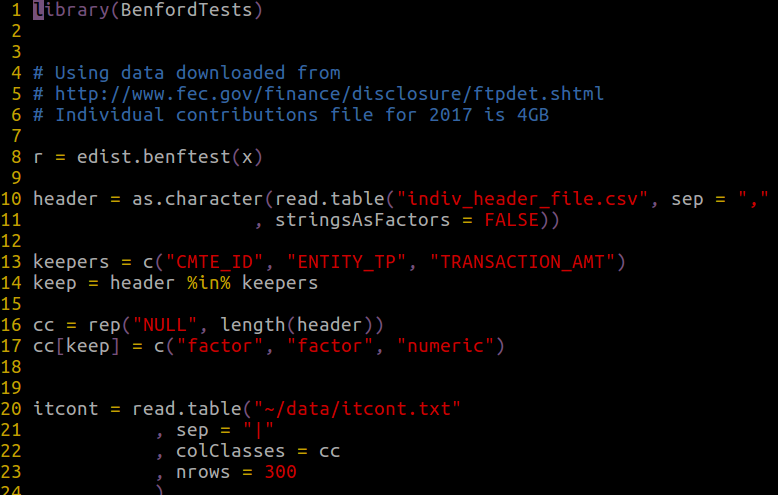
\includegraphics[width=1.4in]{code_screen.png}
            \hfill
            
\includegraphics[width=1in]{database.png}
            \hfill
            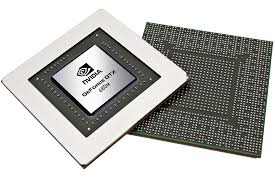
\includegraphics[width=1.4in]{gpu.jpg}
\end{figure}

\end{frame}
%%%%%%%%%%%%%%%%%%%%%%%%%%%%%%%%%%%%%%%%%%%%%%%%%%%%%%%%%%%%
\begin{frame}

    \frametitle{The next step is to build a prototype of the system.}

    Specifically beginning with:

\begin{itemize}
    \item \emph{code}: Apply family of functions
    \item \emph{data}: Files on disk exceeding main memory
    \item \emph{platform}: Single server
\end{itemize}

Then test it with the traffic sensor data.

% My immediate plan is to build a prototype of the system targeting R's apply
% style functions on a single
% server \emph{platform}, and \emph{data} consisting of files on disk which
% may exceed memory. I'll test this prototype on the problem described in
% section~\ref{sec:pems}. At a minimum this means preprocessing tools
% and a parallel tapply / group by.  Once the prototype is functional
% I plan to extend the data model to streaming data through big data systems
% such as Apache Kafka. Running R along with a streaming system is
% interesting and relevant because it allows one to bring the statistical
% power of R beyond the offline analysis of static data and into large real
% time systems. 

\end{frame}
%%%%%%%%%%%%%%%%%%%%%%%%%%%%%%%%%%%%%%%%%%%%%%%%%%%%%%%%%%%%
\begin{frame}

\frametitle{Longer term I'd like to extend this to streaming data.}

% TODO

Running R along with a streaming system is
interesting and relevant because it allows one to bring the statistical
power of R beyond the offline analysis of static data and into large real
time systems. 

\end{frame}
%%%%%%%%%%%%%%%%%%%%%%%%%%%%%%%%%%%%%%%%%%%%%%%%%%%%%%%%%%%%
\begin{frame}

    \frametitle{Acknowledgements}

\begin{itemize}
    \item Faculty members
    \item Data Science Institute Affiliates and statistics students for
        applications and feedback
    \item Special thanks to Professors Duncan Temple Lang and Michael Zhang
\end{itemize}

\end{frame}
%%%%%%%%%%%%%%%%%%%%%%%%%%%%%%%%%%%%%%%%%%%%%%%%%%%%%%%%%%%%
\begin{frame}

    \frametitle{Questions?}
    \centerline{\includegraphics[height=2.5in]{../workflow.pdf}}

\end{frame}
%%%%%%%%%%%%%%%%%%%%%%%%%%%%%%%%%%%%%%%%%%%%%%%%%%%%%%%%%%%%
\begin{frame}

    \frametitle{Additional Slides}

\end{frame}
%%%%%%%%%%%%%%%%%%%%%%%%%%%%%%%%%%%%%%%%%%%%%%%%%%%%%%%%%%%%
\begin{frame}

    \frametitle{More Applications}

    % TODO: Expand on each of these

\begin{itemize}
    \item Benford test on election campaign contribution data
        %\cite{tam2007breaking}
    \item Forest greenness satellite imagery (Andrew Latimer)
    \item Simulating spread of disease (Nistara Randhawa)
\end{itemize}

\end{frame}
%%%%%%%%%%%%%%%%%%%%%%%%%%%%%%%%%%%%%%%%%%%%%%%%%%%%%%%%%%%%
\begin{frame}

    \frametitle{Last summer I worked on the Distributed Data Structures in
R (DDR) project}

% Expert users had some valid critiques and suggestions
% Bryan Lewis- Maybe R is all the API we need?

\begin{itemize}
    \item Relevant experience
    \item Idea: an abstraction layer for distributed and parallel data structures
    \item Created R lists and apply type functions to run on Spark
\end{itemize}


\end{frame}
%%%%%%%%%%%%%%%%%%%%%%%%%%%%%%%%%%%%%%%%%%%%%%%%%%%%%%%%%%%%
\begin{frame}[fragile]

    \frametitle{How do we detect if a function in R is vectorized, and in
    which arguments?}

    \texttt{rnorm()} is vectorized in the last two arguments, but
    semantically different for a vector in the first argument.

\begin{verbatim}
> rnorm(5, mean = c(1, 2), sd = c(2, 10, 200))
[1]   0.2134756  -4.1137221 256.0094734   0.4562226 -10.3855374
\end{verbatim}

It's all C Code.

\begin{verbatim}
> rnorm
function (n, mean = 0, sd = 1)
.Call(C_rnorm, n, mean, sd)
\end{verbatim}

\end{frame}
%%%%%%%%%%%%%%%%%%%%%%%%%%%%%%%%%%%%%%%%%%%%%%%%%%%%%%%%%%%%
\begin{frame}

    \frametitle{An iterator produces data on demand}

    \centerline{\includegraphics[height=1.6in]{../iterator.pdf}}

    \begin{itemize}
        \item Most flexible of the above options
        \item Natural in pipeline parallel model
        \item Operate well with high performance IO libraries
    \end{itemize}

    \pause

    \begin{itemize}
        \item Unfamiliar to R programmers
        \item Not ideal if you need the whole data set
    \end{itemize}

\end{frame}
%%%%%%%%%%%%%%%%%%%%%%%%%%%%%%%%%%%%%%%%%%%%%%%%%%%%%%%%%%%%
\begin{frame}[fragile]

    \frametitle{R in a database}

    Suppose we want to call the vectorized function $f()$. If $f()$ is
    available both in R and the database then we have two options:

\begin{verbatim}
    Option 1: Run f inside database, returning result
    
    dbGetQuery(con,"SELECT f(x) FROM mydata;")

    Option 2: First fetch x, then call f within R

    f(dbGetQuery(con,"SELECT x FROM mydata;"))
\end{verbatim}

\end{frame}
%%%%%%%%%%%%%%%%%%%%%%%%%%%%%%%%%%%%%%%%%%%%%%%%%%%%%%%%%%%%
\begin{frame}[fragile]

    \frametitle{By ``programming on the language'' we can modify existing
    code.}

\begin{verbatim}
lapply_to_mclapply = function(expr)
{
    # Changes lapply to parallel::mclapply
    lapply = quote(parallel::mclapply)
    expr = force(expr)
    # Following Wickham's Advanced R book
    call = substitute(substitute(expr))
    eval(call)
}

> e1 = quote(xmeans <- lapply(x, mean))
> lapply_to_mclapply(e1)
xmeans <- parallel::mclapply(x, mean)
\end{verbatim}

\end{frame}
%%%%%%%%%%%%%%%%%%%%%%%%%%%%%%%%%%%%%%%%%%%%%%%%%%%%%%%%%%%%
\begin{frame}[fragile]

    \frametitle{Pipeline parallelism is like a factory assembly line.}

\centerline{\includegraphics[width=\textwidth]{../pipeline.pdf}}

\begin{verbatim}
# Worker 1
x_chunk = rnorm(n_j)
serialize(x_chunk, worker2)


# Worker 2
x_chunk = unserialize(worker1)
partial_means[i] = mean(x_chunk)
\end{verbatim}

\end{frame}
%%%%%%%%%%%%%%%%%%%%%%%%%%%%%%%%%%%%%%%%%%%%%%%%%%%%%%%%%%%%
\begin{frame}

    \frametitle{Simple row based sampling misses the important areas of high
    density.}

    \centerline{\includegraphics[height=2.5in]{../../analysis/pems/occ_flow_with_sample.pdf}}


%%%%%%%%%%%%%%%%%%%%%%%%%%%%%%%%%%%%%%%%%%%%%%%%%%%%%%%%%%%%
%%%%%%%%%%%%%%%%%%%%%%%%%%%%%%%%%%%%%%%%%%%%%%%%%%%%%%%%%%%%
%%%%%%%%%%%%%%%%%%%%%%%%%%%%%%%%%%%%%%%%%%%%%%%%%%%%%%%%%%%%

\end{frame}
%\begin{frame}
%\frametitle{References}
%\printbibliography
%\end{frame}

\end{document}
